\Chapter{Numerical Experiment}

\Section{Option Pricing}

Option Pricing has always been a challenging topic in financial mathematics. 
Although there are several other methods for pricing options, Monte Carlo performs better when solving high dimension problems.
In this chapter we make several tests our reliable QMC with CV algorithm with option pricing problems. 
Note all our experiments are implemented under brownian motion (GBM) pricing model on non dividend paying stock.  
Since the GBM model is a well known model for option pricing, we only lay out the parameters for option formulas we use later and not dig into the model itself. 
\begin{align*}
    S(jT/d)&=\text{current asset price at time $jT/d,\; j=1,\dots,d$}\\
    K&=\text{strike price}\\
    T&=\text{expiration time}\\
    \sigma&=\text{volatility}\\
    r&=\text{interest rate}\\
    d&=\text{number of time steps}.
\end{align*}

\Subsection{Accuracy}
The first thing we want to test is whether our algorithm provides the `accurate' solution. 
This means if the function satisfies the cone condition, the difference between our estimation and true value should be bounded by the pre-defined error tolerance. 
We will test our algorithm for accuracy in three cases: original reliable adaptive QMC (RAQMC), reliable adaptive QMC with CV (RAQMC\_CV) for single CV and RAQMC\_CV for double CV. 

To do this we have to know the exact value of our integral to calculate the exact error of our results. 
Therefore, we choose the geomatric mean Asian option as our target function because we have the exact pricing formula under GBM model \cite{kemna1990pricing}. 
We choose to test the call options, for the geomatric mean Asian call option the payoff function is:   
\[ C_{T}^{\mathrm{gmean}} = \max\Big(\Big[\prod_{j=1}^{d}S(jT/d) \Big]^\frac{1}{d}-K, 0\Big)e^{-rT}.\]
The closed formula for the exact price under the GBM model is: 
\begin{align}
    C_{T}^{\mathrm{gmeanExact}} 
    &= S(0)e^{-(r+\sigma^2/2)T/2}\Phi(\tilde{d}_1)+Ke^{-rT}\Phi(\tilde{d}_2)    \label{eq:exactgmean}\\
    \tilde{d}_1 &=\frac{\ln(S(0)/K)+(r+\frac{n-1}{6(n+1)}\sigma^2/2)T/2}
    {\sqrt{\frac{2n+1}{6(n+1)}}\sigma\sqrt{T}}\notag\\
    \tilde{d}_2 &=\frac{\ln(S(0)/K)+(r-\sigma^2/2)T/2}
            {\sqrt{\frac{2n+1}{6(n+1)}}\sigma\sqrt{T}}\notag.
\end{align}

Then we need several CV of which the exact solution must have clear formulas. 
Here we pick the European call option and the stock price at expiration as control variates.   
For the European call option, the payoff function is: 
\[ C_{T} = \max (S(T)-K,0)e^{-rT}.\] 
The exact price under the GBM model is given by \cite{boyle1977options}:  
\begin{align*}
    C_{T}^{\mathrm{euroExact}} &= S(0)\Phi(d_1)-Ke^{-rT}\Phi(d_2)\\
    d_1 &=\frac{\ln(S_0/K)+(r+\sigma^2/2)T}{\sigma\sqrt{T}}\\
    d_2 &=\frac{\ln(S_0/K)+(r-\sigma^2/2)T}{\sigma\sqrt{T}}.
\end{align*}
For the stock price, the expected discounted price is $S(T)e^{-rT}$, while the exact price under the GBM model is just $S(0)$.  

\begin{table}[h]
    \centering
	\caption{Parameter Setup for accuracy test}
    \label{tb:accsetup}
	\begin{tabular}{ccccc}
		\hline\hline
        S0 & K & TimeVector & r & volatility \\[0.5ex]
        \hline
        120  & 100 & 1/52:1/52:4/52 & 0.01 & 0.5 \\[1ex] 
        \hline
	\end{tabular}
\end{table}
Table~\ref{tb:accsetup} shows the set up for all options in the accuracy test.
We use the in the money call option for both Asian and European options. 
They are monitored weekly for a one month period with 1\% interest and 50\% volatility anunally. 
\begin{table}[h]
    \centering
	\caption{Accuracy Test of RAQMC\_CV algorithm}
    \label{tb:accuracy}
    \begin{tabular}{lccc}  
    \hline \hline
    abstol = $10^{-2}$ &RAQMC&RAQMC\_CV$_1$&RAQMC\_CV$_2$\\[0.5ex]
    \hline
    exact price& 1.2926641930& 1.2926641930&1.2926641930\\[0.5ex]
    estimate price& 1.2938177355& 1.2937890386&1.2930809161\\[0.5ex]
    err=$|$exact-estimate$|$ & 1.1535e-3& 1.124e-3&4.167e-4\\[0.5ex]
    \hline
    abstol = $10^{-3}$ &RAQMC&RAQMC\_CV$_1$&RAQMC\_CV$_2$\\[0.5ex]
    \hline
    exact price& 1.2926641930& 1.2926641930&1.2926641930\\[0.5ex]
    estimate price& 1.2926529108& 1.2925687148&1.2925793049\\[0.5ex]
    err=$|$exact-estimate$|$ & 1.12821e-5& 9.54782e-5&8.48881e-5\\[0.5ex]
    \hline
    abstol = $10^{-6}$ & RAQMC&RAQMC\_CV$_1$&RAQMC\_CV$_2$\\[0.5ex]
    \hline
    exact price& 1.2926641930& 1.2926641930&1.2926641930\\[0.5ex]
    estimate price& 1.2926643000& 1.2926639635&1.296646297\\[0.5ex]
    err=$|$exact-estimate$|$ & 1.07e-7& 2.295e-7&4.367e-7\\[0.5ex]
    \hline
    \end{tabular}
\end{table}
The test is on three scenarios: RAQMC, RAQMC\_CV with one CV ($\textrm{RAQMC\_CV}_1$) and RAQMC\_CV with two CV ($\textrm{RAQMC\_CV}_2$).
The test is then performed with three different absolute error tolerances as shown in table~\ref{tb:accuracy}.
First we caculated the exact price for the geomatric mean Asian call option using formula~\eqref{eq:exactgmean}. 
Then we run the same parameters through RAQMC\_CV to get the estimates. 
Finally, we caluate the absolute value of difference between estimates and true prices as errors. 
We used three different absolute error tolerance set ups for this: $10^{-2}, 10^{-3}, 10^{-6}$.   
From the results we can see all errors lied within the preset tolerance. 
This give us confidence for our algorithm as accurate as guranteed. 
Note for the second test, which the tolerance is $10^{-3}$, while the error seems all within a lesser bound $10^{-4}$. 
We believe this is not an error for the algorithm or the code.  
It happened since each iteration our sample size is doubled and this could be more than satisfied for the predefined tolerance level.


\Subsection{Efficiency}
Now that we know our algorithm provides the desired results, we continue to test the time efficiency of the algorithm. 
Here we do not use time complexity like big O notation. This is because the results of our algorithm depend not only on dimention but also on target function itself. Since we use an iterative way to stop we can not know the anwer apriori. 
Instead, we do experiments to test the `efficiency' of our algorithm by compare the sample size used for caculation and the corresponding time cost. 
Note the results do not stay the same for each time, to compensate that we take an average of 10 consecutive runs with the same set-up. 
This test breaks into two parts. 
The first one is that we want to know how our algorithm performs without using CV. 
Naturally the RAQMC algorithm we introduced in chapter 3 become a good reference. 
We know our algorithm is a bit slower compared to it when not using CV. The question is how small the gap is. 
If there is no significant difference, then it means we will not waste too much time on cases without CV or with poor CV. 
The second one, which is more important, is that we want to see how much time it can save by using good CV. Of course this depends on quality of the CV. Fortunately, several good CV is known to be use for option pricing under GBM model \cite{lidebrandt2007variance}.         

\Subsubsection{RAQMC\_CV without CV}
Parameter set up for efficiency test is shown in table~\ref{tb:effsetup}. 
This time we try to price a daily monitored four months period option, which increases the dimension to 64. 
Note we will keep using this set up for all the following efficienty tests. 
\begin{table}[h]
    \centering
	\caption{Parameter Setup for all efficienty tests}
    \label{tb:effsetup}
	\begin{tabular}{ccccccc}
		\hline\hline
        S0 & K & TimeVector & r & volatility & abstol & reltol \\[0.5ex]
        \hline
        120  & 130 & 1/250:1/250:64/250 & 0.01 & 0.5 & 1e-3 & 0\\[1ex] 
        \hline
	\end{tabular}
\end{table}
We test our algorithm through four scenarios: RAQMC, RAQMC\_CV without CV ($\textrm{RAQMC\_CV}_0$), 
RAQMC\_CV with one poor CV ($\textrm{RAQMC\_CV}_1$) and RAQMC\_CV with two poor CV ($\textrm{RAQMC\_CV}_2$). 
For target option we still use geomtric mean Asian option European option. For single CV we use European option and add stock price for double CV. 
\begin{table}[h]
    \centering
	\caption{Efficiency test I of RAQMC\_CV}
    \label{tb:efftest1}
    \begin{tabular}{lcccc}  
    \hline\hline
    \hline
    abstol$=10^{-3}$&RAQMC&RAQMC\_CV$_0$&RAQMC\_CV$_1$& RAQMC\_CV$_2$\\[0.5ex]
    \hline
    Sample Size	&65535&65535&65535&65535\\[1ex]
    Time Cost &1.8365&1.8379 &1.8808 &1.8703\\[1ex]
   \hline
	\end{tabular}
\end{table}
As shown in table~\ref{tb:efftest1}, all test end up with same sample size, which means that choice of CV didn't help at all. 
But what we concern is that how much extra cost can it bring if our choice of CV is bad? We can see the time cost just increased around 2\% for QMC with bad CV. Now we can say our method did make the cost of CV to a minimal.  

\Subsubsection{RAQMC\_CV with CV}
\begin{table}[h]
    \centering
	\caption{Efficiency test II of RAQMC\_CV algorithm with Asian Option}
    \label{tb:efftest2a}
    \begin{tabular}{lcccc}  
    \hline\hline
    &Estimate Price&Sample Size&Time Cost&$\beta^*$\\[0.5ex]
    \hline
    RAQMC& 4.2011&65535 & 1.9054 & null\\[1ex]
    RAQMC\_CV$_1$&4.2008& 15564.8 & 0.49966& 0.995 \\[1ex]
    RAQMC\_CV$_2$&4.2018& 13926.4 & 0.43793&(0.958,0.005)$^T$\\[1ex]
    \hline
	\end{tabular}
\end{table}
There are two types of asian options, depends on which types of mean one use. 
In last section we introduced geomatric mean Asian option, this time we choose arithematic mean asian call option as our target function, whose payoff function is:
\[ C_{T}^{Amean} = \max\Big(\frac{1}{d}\sum_{j=1}^{d}S(jT/d)-K, 0\Big)e^{-rT}.\]
For this option there is no close formula for exact price under GBM model.
However, recall we introduced another Asian option earlier of which the price has a clear formula. 
It is known that geomatric mean Asian option was first used as a CV for pricing arithmatic mean Asian option \cite{kemna1990pricing}. 
Hence, for single CV we choose geomatric mean Asian call option as CV. 
We also want to test it for double CV so we add European call option as a second CV. 
Results are shown in table~\ref{tb:efftest2a}. We can see this choice of CV is really good. 
The sample size is approximately $1/4$ of original size and same with time cost. 
The second CV didn't make an obvious improvement compared to single CV but seems helped a bit.    

\begin{figure}[h]
    \centering
    %\setlength{\unitlength}{0.14in}     % selecting unit length
    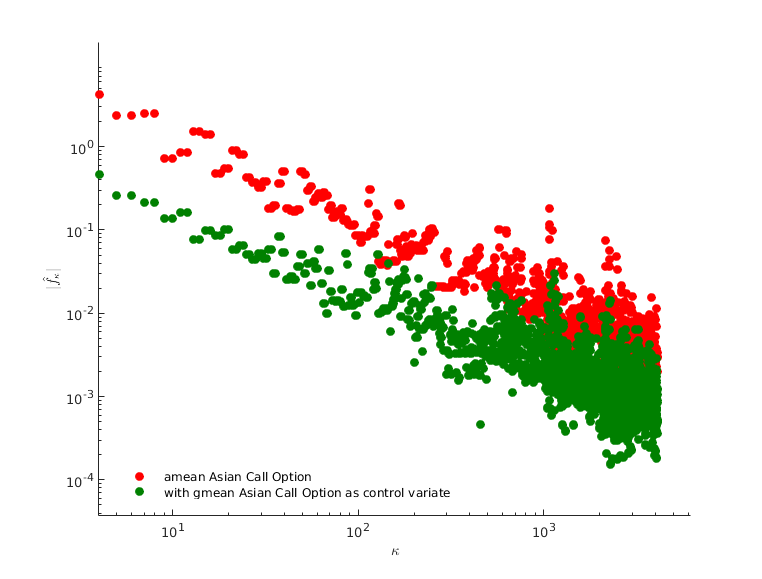
\includegraphics[width=\textwidth]{figures/cvEx1.eps}
    \caption{Walsh coefficients of $f$}
    \label{fg:cvEX1}
\end{figure}

Figure~\ref{fg:cvEX1} is a plot of the walsh coefficients for the target function and control variates in this Asian options experiments. Recall our error of approximation is bound on this exact same coeffcients. 
What we'd expect is that on both method it can decrease fast and for CV method we expect it to decrease faster.   
The horizontal axis in the figure can be interpreted as sample size, the vertical axis can be view as the error bound. What our algorithm does is that for a give error bound, we monitor these Walsh coefficients untill it reaches the bound. Obviously, the CV method will stop early in this case which means less compuational cost for it. 

Another good example is barrier option. This is the payoff function for up and in barrier call option:
\[ C_{T}^{\mathrm{U\&I}} = [S(T)-K]^+1_{ \{\max{S(jT/d)}\geq \mathrm{Barrier}\}}.\]
The reason we choose it is for its similaritis to the European option. 
Note if the barrier equals strike price (130), then it is just a European call option, which makes european option a good control variates.
For this test we take four different barriers that gradually decrease to the strick price. 
We use the same parameter set-up as the previous one which is shown in table~\ref{tb:effsetup}. 
As same as the last test, we compared oringinal RAQMC algorithm and RAQMC\_CV on sample size and time cost. 
\begin{table}[h]
    \centering
	\caption{Efficiency test II of RAQMC\_CV algorithm with Barrier Option}
    \label{tb:efftest2b}
    \begin{tabular}{lccccc}
    \hline\hline
	Barrier &\multicolumn{2}{c}{Sample Size}
		&\multicolumn{2}{c}{Time Cost}
        &$\beta^*$ \\
    \hline
	&RAQMC&RAQMC\_CV
    &RAQMC&RAQMC\_CV\\[0.5ex]
    \hline
	160  & 1048576&1048576 
    & 49.9861&50.8245 &0.6613 \\ 
	150  & 1048576&524288 
    & 47.8742&23.2743 &0.8999 \\ 
	140  & 524288&32768
    & 22.7936&1.0146 &0.9935\\ 
	130  & 524288&1024
    & 22.3675& 0.0826 &1.0000 \\[1ex]
    \hline
	\end{tabular}
\end{table}
One merit for this example is that we can see how the cost and value of $\beta^*$ change as we change the barrier. 
In this example we know the optimal value should be close to $1$ as shown in table~\ref{tb:efftest2b} when barrier=130. 
Also, note we set the start sample size for iteration to be $2^{10}$, which is exactly the sample size used in this case. 
This is consistant with our statement earlier, it is just a European option. 
When we move barrier further from 130, we assume the European option will not be as good as the pervious one as a CV\@. 
Our results confirmed this assumption, we can see in table~\ref{tb:efftest2b} both the time cost and sample size rise as we increase the barrier. 
At last when barrier=160, European option completely lost its value as CV and cost of two methods are almost the same. 

\newpage
\Section{Multivariate normal probabilities}

For this part tests, we are interested in computing the probability of a multivariate normal distribution in dimension 6
\[
    F([0,1)^6)=\int_{[0,1)^6}\frac{1}{\sqrt{|\Sigma|(2\pi)^6}}
        e^{\frac{1}{2}\mathbf{x}^T\Sigma^{-1}\mathbf{x}}
        \;\textrm{d}\mathbf{x},
    \]
where $\Sigma$ is a symmetric positive definite covariance matrix. 
So this time the target function is multivariate normal density function and to make it simple we set the covariance matrix in the following form 
\[
    f(\mathbf{x})= \frac{1}{\sqrt{|\Sigma|(2\pi)^6}}
        e^{\frac{1}{2}\mathbf{x}^T\Sigma^{-1}\mathbf{x}},\;
\Sigma=
\begin{pmatrix}
    1&\sigma&\sigma&\sigma&\sigma&\sigma\\[-1.5em]
    \sigma&1&\sigma&\sigma&\sigma&\sigma\\[-1.5em]
    \sigma&\sigma&1&\sigma&\sigma&\sigma\\[-1.5em]
    \sigma&\sigma&\sigma&1&\sigma&\sigma\\[-1.5em]
    \sigma&\sigma&\sigma&\sigma&1&\sigma\\[-1.5em]
    \sigma&\sigma&\sigma&\sigma&\sigma&1
\end{pmatrix}.
\]
Then we choose the two multivariate normal distribution with diagonal covariance matrices as CV 
\begin{align*}
&h_1(\mathbf{x})= \frac{1}{\sqrt{|\Sigma_1|(2\pi)^6}}
        e^{\frac{1}{2}\mathbf{x}^T\Sigma_1^{-1}\mathbf{x}},\;
    \Sigma_1=
\begin{pmatrix}
    1&0&0&0&0&0\\[-1.5em]
    0&1&0&0&0&0\\[-1.5em]
    0&0&1&0&0&0\\[-1.5em]
    0&0&0&1&0&0\\[-1.5em]
    0&0&0&0&1&0\\[-1.5em]
    0&0&0&0&0&1
\end{pmatrix}\\
&h_2(\mathbf{x})= \frac{1}{\sqrt{|\Sigma_2|(2\pi)^6}}
        e^{\frac{1}{2}\mathbf{x}^T\Sigma_2^{-1}\mathbf{x}},\;
\Sigma_2=
\begin{pmatrix}
    \sigma&0&0&0&0&0\\[-1.5em]
    0&\sigma&0&0&0&0\\[-1.5em]
    0&0&\sigma&0&0&0\\[-1.5em]
    0&0&0&\sigma&0&0\\[-1.5em]
    0&0&0&0&\sigma&0\\[-1.5em]
    0&0&0&0&0&\sigma
\end{pmatrix}.
\end{align*}
The reason we pick these as CV is that they are from the same multivariate gaussion family and correlate to the targe function. 
Computation of the integrals on these CV are rather simple since each dimension is independent in this case. But still the $\theta$ we computed is an approximation and this introduce a bias into our estimator. 
We think the results can still be useful since the error for $\theta$ is rather small and we can do it fast.

We choose three different value for $\sigma$ ($0.1, 0.4$ and $0.7$) and run the test for three senarios: RAQMC, RAQMC\_CV with h1 as CV (RAQMC\_CV$_1$), RAQMC\_CV with h1 and h2 as CV (RAQMC\_CV$_2$). 
\begin{table}[h]
    \centering
	\caption{Test of RAQMC\_CV with multivariate normal probability}
    \label{tb:mvntest}
    \begin{tabular}{lccc}  
    \hline \hline
    $\sigma=0.1$, abstol=$10^{-7}$ &RAQMC&RAQMC\_CV$_1$&RAQMC\_CV$_2$\\[0.5ex]
    \hline
    estimate value& 0.0020706728& 0.0020706626&0.0020706649\\[0.5ex]
    err=$|$`exact'-estimate$|$ & 1.8e-9&4.3e-9&7.0e-9\\[0.5ex]
    sample size& 27852& 4096&4096\\[0.5ex]
    time cost& 0.0414& 0.0206&0.0242\\[0.5ex]
    $\beta^*$& null&1.1093 & (0.9649,4.47e-5)$^T$\\[0.5ex]
    \hline
    $\sigma=0.4$, abstol=$10^{-7}$ &RAQMC&RAQMC\_CV$_1$&RAQMC\_CV$_2$\\[0.5ex]
    \hline
    estimate value& 0.0046138363& 0.0046138346&0.0046138341\\[0.5ex]
    err=$|$`exact'-estimate$|$ & 1.9e-9& 1.9e-9&2.6e-9\\[0.5ex]
    sample size& 65536& 32768&32768\\[0.5ex]
    time cost& 0.0805&0.0595&0.0628\\[0.5ex]
    $\beta^*$& null&2.2582 & (0.9673,0.0408)$^T$\\[0.5ex]
    \hline
    $\sigma=0.7$, abstol=$10^{-7}$& RAQMC&RAQMC\_CV$_1$&RAQMC\_CV$_2$\\[0.5ex]
    \hline
    estimate value&0.0169509335 & 0.0169509327&0.0169509342\\[0.5ex]
    err=$|$`exact'-estimate$|$ & 1.8e-9& 6.1e-9&3.6e-9\\[0.5ex]
    sample size& 524288& 511180&262144\\[0.5ex]
    time cost& 0.5235& 0.6187&0.3626\\[0.5ex]
    $\beta^*$& null&8.6074 &(-18.95,7.78)$^T$\\[0.5ex]
    \hline
    \end{tabular}
\end{table}
The sample size and time cost in table~\ref{tb:mvntest} are average value from 20 identical runs. 
Because the exact value of the target integral is unknown, we use an approximation for `exact' value to compute the error. 
These approximations are computed using a method developed by Genz and Bretzwith an error of $10^{-10}$ \cite{genz1992numerical}. 
Similarly, we computed the mean of CV with the method developed by Drezner and Wesolowsky and by Genz \cite{drezner1978computation}\cite{genz2004numerical}. The time cost for computation of means of CV is included in the results.  

We start the test with $\sigma=0.1$. 
With this setting the targe function should be close to the first CV. 
As expected, both single and double CV perform great. The sample size is reduced to $4096$ from $27852$ and time cost is about half down compared to RAQMC. 
As we increase the value of $\sigma$, the first CV start to lose its value. 
When $\sigma=0.7$ the first CV become not helpful and cost more time than RAQMC. In the mean time, the double CV method show some good effect, at $\sigma=0.7$, the sample size is half of the other 2 and time cost is about 30\% lesser.

